\documentclass{article}
\usepackage[a4paper]{geometry}
\usepackage{graphicx}
\usepackage[export]{adjustbox}
\geometry{textwidth=\paperwidth, textheight=\paperheight, noheadfoot, nomarginpar}
\setlength{\topskip}{3cm}
\setlength{\parindent}{0mm}
\begin{document}
\begin{center}
\textsc{\textbf{\huge{Abhishek Kaushal}}}
\end{center}
\noindent\makebox[\linewidth]{\rule{17cm}{1.8pt}}

\begin{table}[h!]
  \begin{center}
    \begin{tabular}{l p{4cm} l} 
      \textbf{520-B Madhuban Colony} &  & \textbf{Contact: 08010095277}       \\ 
	\textbf{Kulesara, Greater Noida} &  & \textbf{e-mail id:abhishekkaushal1996@gmail.com}\\
	\textbf{G.B. Nagar, U.P.}&  &\\
	\textbf{201306}
    \end{tabular}
  \end{center}
\end{table}

\begin{figure}[h]
\advance\leftskip-68mm
\noindent
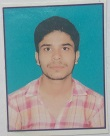
\includegraphics[scale=0.7,right]{IMG_20171204_155357.jpg}
\end{figure}

\begin{table}[h!]
  \begin{center}
    \begin{tabular}{l  l} 
      \textbf{\Large{OBJECTIVE}}\\ \textbf{\Large{EDUCATION}} & 
	
          \begin{tabular}{| c | c | c | c | c |} 
		\hline
     	 	\textbf{Degree} & \textbf{College/School} & \textbf{University} & \textbf{Passing Year} & \textbf{Pass Percentage}\\
		\hline
		B.Tech. & AKTU  & MGM College of Engineering & 2014-2018 & 74 \% \\
		 && and Technology, NOIDA &&\\
		\hline
		$12^{th}$(Science) & CBSE  & Cambridge School  & 2014 & 85.8 \% \\
		&&Greater Noida &&\\
		\hline
		$10^{th}$ & CBSE  & Cambridge School  & 2014 &  81\% \\
		&&Greater Noida &&\\
		\hline
   	 \end{tabular}
 	 
    \end{tabular}
  \end{center}
\end{table}

\begin{table}[h!]
    \begin{tabular}{l  p{2.4\textwidth}} 
      \textbf{\Large{PROJECTS}} & 
	\begin{enumerate}
	\item Transport Management System – Web App, Android app and TED (Trucking Electronic Device)
	\item Care India – Health Survey Android app (Smart India Hackathon 2017)
	\item Propeller Display (Forming pattern using LED bar)
	\item Digital attendance App
	\item Record Management System using Swing and MySQL
   	\end{enumerate} 
    \end{tabular}
\end{table}

\begin{table}[h!]
    \begin{tabular}{l  p{2.4\textwidth}} 
      \textbf{\Large{TRAINING \&}} \\  \textbf{\Large{INTERNSHIP}}& 
	\begin{itemize}
	\item 1 Month Trainee in R\& D Department at Videotex International Pvt. Ltd.
	\item 3 days workshop by IIT Bombay on firebird V.
	\item 6 Months training on core and andvance JAVA at Ducat India
	\item Online training on Python 3
   	\end{itemize} 
    \end{tabular}
\end{table}

\begin{table}[h!]
    \begin{tabular}{l  p{2.4\textwidth}} 
      \textbf{\Large{RESEARCH \&}} \\  \textbf{\Large{PUBLICATIONS}}& 
	\begin{enumerate}
	\item Request for paper publish in IEEE transportation management system.
	\item Ongoing research on Genetic Algorithm.
   	\end{enumerate} 
    \end{tabular}
\end{table}

\begin{table}[h]
    \begin{tabular}{l  p{2.4\textwidth}} 
      \textbf{\Large{TECHNICAL}} \\  \textbf{\Large{SKILLS}}& 
	\begin{itemize}
	\item \textbf{Languages: } C/C++, Core \& advance Java, Struts framework,PHP,Collection framework, Python
	\item \textbf{Databases: } MySQL, oracle and MongoDB
	\item \textbf{Tools: }Arduino IDE, Multisim, Atmel Studio, Microsoft Office,Eclipse,Netbeans
	\item \textbf{Hardware: }SIM 808 Module (GSM/GPS/GPRS), R305 Fingerprint sensor, Arduino Uno \& Mega,etc
	\item \textbf{Operating System: }Windows-XP, Vista, 7, 8, 8.1, 10, Ubuntu, kali
   	\end{itemize} 
    \end{tabular}
\end{table}

\begin{table}[h!]
    \begin{tabular}{l  p{2.4\textwidth}} 
      \textbf{\Large{SOFT SKILLS}} & 
	\begin{enumerate}
	\item Planning and Time Managemet.
	\item Technology Trend Awareness.
	\item Problem Solving
	\item Emotional Intelligence and Stress Management.
	\item Adaptibility and Competitiveness.
   	\end{enumerate} 
    \end{tabular}
\end{table}

\begin{table}[h]
    \begin{tabular}{l  p{2.4\textwidth}} 
      \textbf{\Large{EXTRA-}} \\  \textbf{\Large{CURRICULAR}}\\ \textbf{\Large{ACTIVITIES}}&
	\begin{itemize}
	\item Envirnment Head at School level
	\item Conducted worshop on Fire Bird V at college level
	\item Volunteer at E-Yantra teacher's workshop
	\item Vice head of E-Yantra at college
   	\end{itemize} 
    \end{tabular}
\end{table}

\end{document}